\documentclass[11pt,a4paper]{article}
\usepackage[main=ngerman,russian]{babel}
\usepackage{ls}
\usepackage[utf8]{inputenc}
\usepackage{hyperref}

\title{Handout -- Evolutionbäume technischer Systeme\\ bei Nikolay Shpakovsky}

\author{Tom Strempel}
\date{19.01.2021}

\begin{document}

\maketitle

\section{Einleitung}
% Objekt (übt für uns allein keine nützliche Funktion aus) <-> Komponete

Das Buch \emph{Tree of Technology Evolution} erschien 2016 als Übersetzung des
russischen Originals von 2010, welches von Nikolay Shpakovsky verfasst wurde.
Darin werden die Konzepte des Evolutionsmusters und Evolutionsbaumes
eingeführt, um Informationsfelder zu strukturieren.

Shpakovsky hat diese Konzepte auf der Basis der Analyse einer großen Menge
realer technischer Systeme entwickelt. Die Gesetze der TRIZ sind auf dieselbe
Weise entstanden, und Altschullers Arbeit stellt auch die Grundlage für
Shpakovsky dar.

Die ersten drei Kapitel des Buches beschäftigen sich mit den Grundlagen zum
Erstellen der Evolutionsbäume. In den darauffolgenden Kapiteln wird die
Erstellung und Anwendung von Evolutionsbäumen thematisiert.

\section{Begriffsdefinitionen}

Es erfolgt eine Schärfung des Idealitätsbegriffs eines technischen Systems.
Laut Shpakovsky ist ein ideales System ein System, welches seine Funktion mit
vernachlässigbaren Kosten in Bezug auf den Nutzen ausführen kann. Die
Ausführungskosten $C$ können aber nicht null betragen. Das Ziel der
technischen Evolution ist es, ein möglichst ideales System zu erzeugen.

Im Buch wird die verrichtete Arbeit $F$ einer Funktion als \emph{Performance}
bezeichnet. Dieser Begriff ist aus meiner Sicht schon durch das
Leistungsverhalten einer Software belegt, demnach wird folgend $F$ als
verrichtete \emph{Arbeit}\footnote{Gräbe: Der Parameter auf der Ordinate des
  Diagramms einer S-Kurve wird in der deutschen Literatur (etwa
  Koltze/Souchkov) oft als \emph{Leistung} oder \emph{Nutzen} bezeichnet.  Der
  Parameter bleibt ähnlich vage und qualitativ wie das gesamte
  S-Kurven-Konzept.  \emph{Arbeit} ist ein wenig tauglicher Begriff, da er
  sich physikalisch als Leistung mal Zeit berechnet.}  einer Funktion
definiert.

\begin{equation*}
  I = \frac{F}{C}
\end{equation*}
Mit:
\begin{itemize}[noitemsep]
\item $I$: Idealität
\item $F$: Verrichtete Arbeit der Funktion
\item $C$: Ausführungskosten der Funktion
\end{itemize}

Eine Funktion ist definiert durch die Ausübung einer Aktion durch ein
Arbeitswerkzeug an einem Arbeitsobjekt.

Es werden drei Problemtypen im modernen Ingenieurwesen identifiziert:
\begin{enumerate}[noitemsep]
\item Lösung dringender technischer Probleme,
\item Vorhersage der zukünftigen Entwicklung technischer Systeme,
\item Patente umgehen bzw. absichern.
\end{enumerate}

Die Behandlung von Patenten und deren Umgehung ist ein wichtiges Motiv im Buch
von Altschuller, da er in seiner Karriere oft darauf zurückgreifen musste.
Dies unterscheidet ihn auch von den bisher behandelten Autoren der TRIZ.  Für
die Lösung dieser drei Problemtypen wird eine \emph{strukturierte
  Wissensbasis} bzw. ein \emph{strukturiertes Informationsfeld} benötigt. Für
ein solches Feld werden fünf Anforderungen von Shpakovsky genannt:

\begin{enumerate}[noitemsep]
\item Objektivität der Klassifikationskriterien
\item Vollständigkeit (Das Vorhandensein aller sich signifikant
  unterscheidenden Versionen)
\item Geeigneter Generalisierungsgrad
\item Visualisierbarkeit
\item Ausreichende Beschreibung bzw. Voraussage noch nicht existierender
  Versionen
\end{enumerate}

\subsection{Keine Gesetze, sondern Empfehlungen}

Shpakovsky spricht bei den aufgestellten Konzepten des Evolutionsmusters und
-baums nie von \emph{Gesetzen}, sondern von \emph{Anforderungen},
\emph{Regeln} und insbesondere bei Konstruktionsanleitungen von
\emph{Empfehlungen}.  Dabei weicht er die Objektivität eigenhändig auf. Eine
wirklich explizite Erklärung dieses Wandels vom Gesetz zur Empfehlung findet
nicht statt, der Umstand kann aber anhand des erstellten Evolutionsbaums des
Bildschirms nachvollzogen werden.  Der Stamm eines Evolutionsbaumes sollte
beispielsweise nur aus einem Evolutionsmuster bestehen
(vgl. \cite[S. 122f]{evo}), es wird aber deutlich, dass beim Bildschirm zwei
Evolutionsmuster als Stamm dienen, nämlich das Trimmen und das Segmentieren.
Hier ist es, aufgrund der Beschaffenheit des betrachteten technischen Systems,
angebracht, die Empfehlung nicht zu befolgen. Dies wäre bei einem Gesetz nicht
möglich bzw. es dürfte gar nicht aufgrund der Natur eines Gesetzes vorkommen.

\section{Evolutionsmuster}

\begin{enumerate}[noitemsep]
\item Mono-Bi-Poly
\item Trimmen
\item Expandieren und Trimmen
\item Segmentierung
\item Evolution von Oberflächeneigenschaften
\item Evolution von inneren Strukturen
\item Geometrische Evolution
\item Dynamisierung
\item Erhöhung der Kontrollierbarkeit\footnote{Gräebe -- russ:
  \foreignlanguage{russian}{управляемость}, engl: controllability, dt besser:
  Steuerbarkeit.} 
\item Erhöhung der Koordination der Aktionen\footnote{Gräbe -- Da das erst im
  Obersystem koordiniert werden kann, wurde dieser letzte Punkt in späteren
  Versionen herausgenommen.}
\end{enumerate}

Aus diesen zehn grundlegenden Evolutionsmustern können spezifischere
Evolutionsmuster erstellt werden. Die Evolutionsmuster von eins bis vier sind
Muster, welche Ressourcen für andere Evolutionsmuster bereitstellen. Es ist
z. B. nicht möglich einen unsegmentierten Monolith zu dynamisieren. Die
Struktur des Objektes wird durch die Muster fünf bis sieben vorgegeben. An
sinnvoll erscheinenden Punkten werden Muster zur Dynamisierung,
Kontrollierbarkeit und Koordination eingefügt. Diese hierarchische Struktur
der Transformationen ist in Abb. \ref{fig:basic_evo} verdeutlicht.

\begin{figure*}[htb]
  \centering
  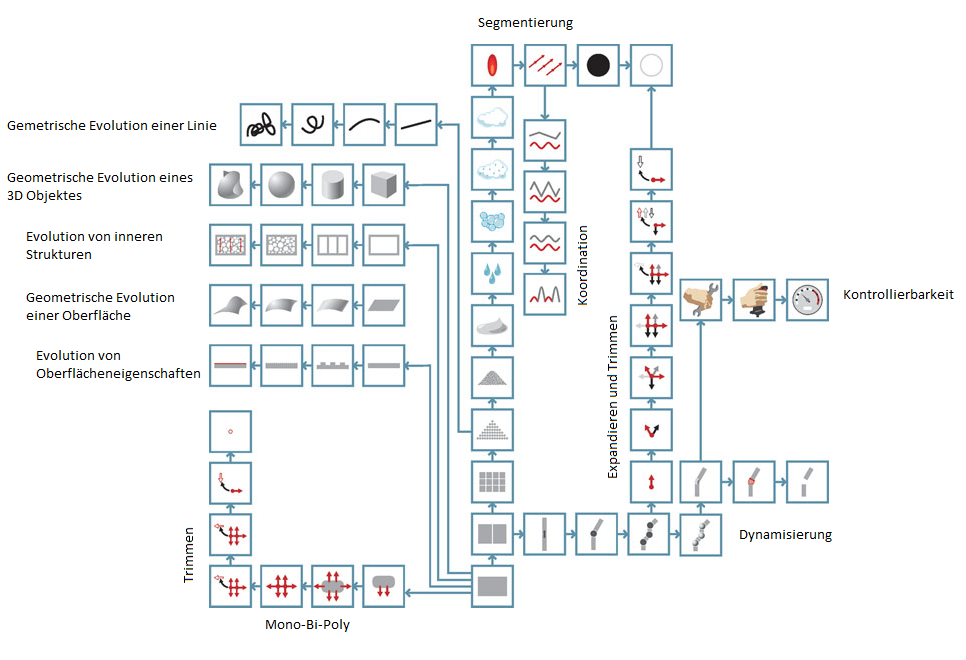
\includegraphics[width=0.9\linewidth]{Basisevolutionsbaum2.png}
  \caption{\small Grundlegender Evolutionsbaum \cite{evo}}
  \label{fig:basic_evo}
\end{figure*}

Eine Transformation ist die Anwendung eines Evolutionsmusters auf ein
\emph{Objekt}, welches darauf folgend zu einer transformierten Version des
Objektes wird.

\section{Evolutionsbaum}

Es existieren grundlegende und spezifische Evolutionsbäume. Grundlegende
Evolutionsbäume stellen eine in einem Baum organisierte Menge von
Evolutionsmuster generalisierter Eigenschaften technischer Objekte dar. Der
Start erfolgt von der simpelsten Version des Objektes z. B. ein Monolith. Die
Hauptachse der Entwicklung wird auch als Stamm bezeichnet, als Stamm werden
Ressourcen bereitstellende Evolutionsmuster wie die Segmentierung bevorzugt,
da diese die Bedingung sind für eine spätere Dynamisierung.


\subsection{Erfüllung der Anforderungen an ein strukturiertes Informationsfeld}

Die behandelnden Konzepte decken alle gestellten Anforderungen an ein
strukturiertes Informationsfeld ab. Objektivität ist gewährleistet durch die
Herleitung von einer großen Menge realer Systeme ähnlich wie in der
TRIZ. Durch die Verwendung des grundlegenden Baums für das Finden aller
Basisversionen eines Objektes ist die Vollständigkeit gewährleistet. Für eine
geeignete Abstraktion btw. Spezifizität wird je nach Anforderung ein
grundlegender oder spezifischer Evolutionsbaum verwendet. Die
Visualisierbarkeit ist gewährleistet durch die Baumstruktur. Lücken bzw. nicht
vollendende Evolutionsmuster können durch einen Vergleich der grundlegenden
und spezifischen Evolutionsbäume gefunden und beschrieben werden.

\subsection{Ermittlung nach nicht bekannter Versionen}
\begin{figure*}[htb]
  \centering
  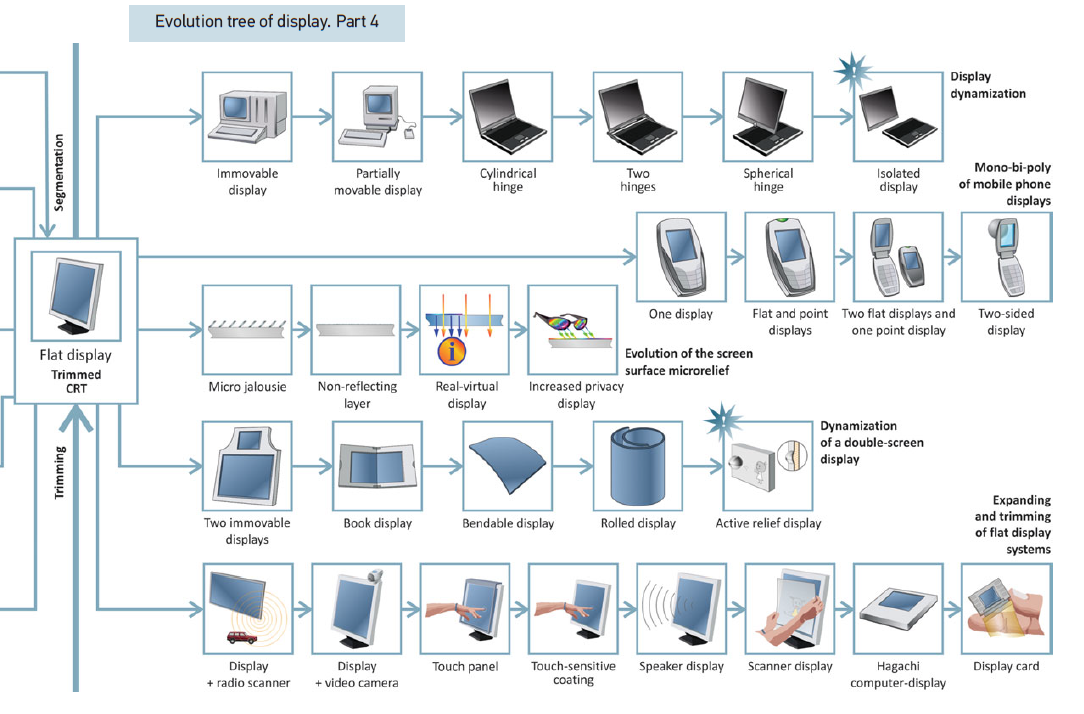
\includegraphics[width=0.9\linewidth]{display.png}
  \caption{\small Ausschnitt des spezifischen Evolutionsbaums vom Bildschirm
    \cite{evo}, siehe \url{http://www.target-invention.com/} für den
    kompletten Baum}
  \label{fig:spez_evo}
\end{figure*}

Für die Analyse eines Objektes muss sowohl der grundlegende (siehe
Abb. \ref{fig:basic_evo}) als auch der spezifische Evolutionsbaum (siehe
Abb. \ref{fig:spez_evo}) erstellt werden. Durch den Vergleich der beiden Bäume
können sowohl Lücken als auch nicht zu Ende geführte Evolutionsmuster entdeckt
werden. Die höchste Stufe des Musters der Dynamisierung besteht aus einer
kompletten Entkopplung der einzelnen Bestandteile. Bei einem Laptop würde dies
bedeuten, dass man Bildschirm und Peripheriegeräte trennen kann. Zur Zeit der
Erstellung des Evolutionsbaums des Bildschirms um 2002 gab es diese Version
des Objektes noch nicht. Durch Erkennung dieser Lücke wurde eine sinnvolle
neue Version gefunden. Die komplette Dynamisierung wird heutzutage erreicht,
indem die Rechentechnik in den Bildschirm integriert wird und die Peripherie
über Bluetooth verbunden wird. Damit wurde gezeigt, dass Evolutionsbäume in
der Lage sind zukünftige Entwicklungen abzubilden.

\section{Patentumgehung}

Es besteht oft das Problem, dass es für ein gewünschtes Produkt bereits ein
Patent gibt. In dieser Situation ist es entweder möglich, hohe Lizenzkosten an
den Patentinhaber zu zahlen oder das Patent zu umgehen.  Die juristische
Methode der Patentumgehung, welche darin besteht, Schlupflöcher und
fehlerhafte Patentbeschreibungen zu nutzen, um ein Patent zu invalidieren, ist
nicht immer anwendbar.  Es ist alternativ möglich, das untersuchte Objekt
abzuändern, um ein besseres Produkt zu entwickeln. Diese erfinderische Methode
hat den Nachteil, dass man hohe Entwicklungskosten hat und den grundlegenden
Aufbau ändern muss. Andererseits ist es nicht möglich, ohne Abänderung ein
alternatives Patent zu bekommen.  Aus diesem für die TRIZ typischen Konflikt
geht eine Synthese in Form der juristisch-erfinderischen Methode hervor. Diese
neue Methode zielt darauf ab, durch Evolutionsbäume noch nicht von Patenten
abgedeckte Transformationsversionen zu finden.  Die Suche nach existierenden
Patenten kann zusätzlich erleichtert werden, indem man die Objekt- und
Transformationsnamen als Schlüsselworte verwendet.

\section{Diskussion}

Folgende Punkte können weiterführend diskutiert werden:
\begin{itemize}[noitemsep]
\item Sind Evolutionsbäume auch für Organisationsstrukturen geeignet?
\item Eigene Ideen zum Evolutionsbaum
\item Shpakovsky nutzt Empfehlungen statt Konzepte, steht damit das Konzept
  der Evolutionsbäume auf wackeligen Füßen?
\end{itemize}

Erläuterung zum ersten Punkt: Shpakovsky verwendet bei der Beschreibung des
Mono-Bi-Poly Evolutionsmusters das Beispiel eines (vgl. \cite[S. 77]{evo})
Schiffgeschwaders. Ein Geschwader, bestehend aus mehreren Schiffen unter einem
gemeinsamen Befehlshaber, stellt ein Poly-System dar. Da es sich dabei aber
nicht definitiv um ein technisches System, sondern um eine Organisationsform,
handelt, stellt sich die Frage, ob Evolutionsbäume auch geeignet sind, 
Organisationsstrukturen darzustellen.

% 2D --> Baum
% Schärfung des Idealitätsbegriffs

%\bibliographystyle{unsrt}
\begin{thebibliography}{xx}
\bibitem{evo} Nikolay Shpakovsky. \emph{Tree of Technology Evolution}. Target
  Invention, 2016.
\end{thebibliography}

\end{document}
